\section{Results}\label{sec:results}

\subsection{Validation of semantic stratification approach for selecting training samples}\label{sec:results:semantic_stratification}

The distribution of the two principal components (PCs) derived from the NLCD histograms for the CBW region in Virginia are shown in Figure~\ref{fig:va_pcs}.
Principal component 1 (PC1) explains \num{66.21}\% of the variance in the data, while principal component 2 (PC2) explains \num{29.11}\% of the variance, for a total of \num{95.32}\% of the variance explained by the first two PCs.
PC1 appears to primarily distinguish candidate patches based on thier urban land cover content - patches with larger positive values of PC1 tend to be placed near urban or built-up regions.
On the other hand, PC2 regions tend to correlate with more vegetated areas.
A qualitative analysis of samples pulled from clusters of PC1 and PC2 are also demonstrated in Figure~\ref{fig:va_pcs}, demonstrating that samples within the same cluster/stratum tend to have similar land cover characteristics.
For example, samples in cluster 50 have a high degree of urban land cover, while samples in cluster 210 have a mix of forested and agricultural land cover.
This pattern is not necessarily fully consistent: for example, most samples in cluster 122 contain a mix of water and forested land cover, but one sample contains no water at all.

\begin{figure}[H]
    \centering
    % \vspace{-0.75cm}
    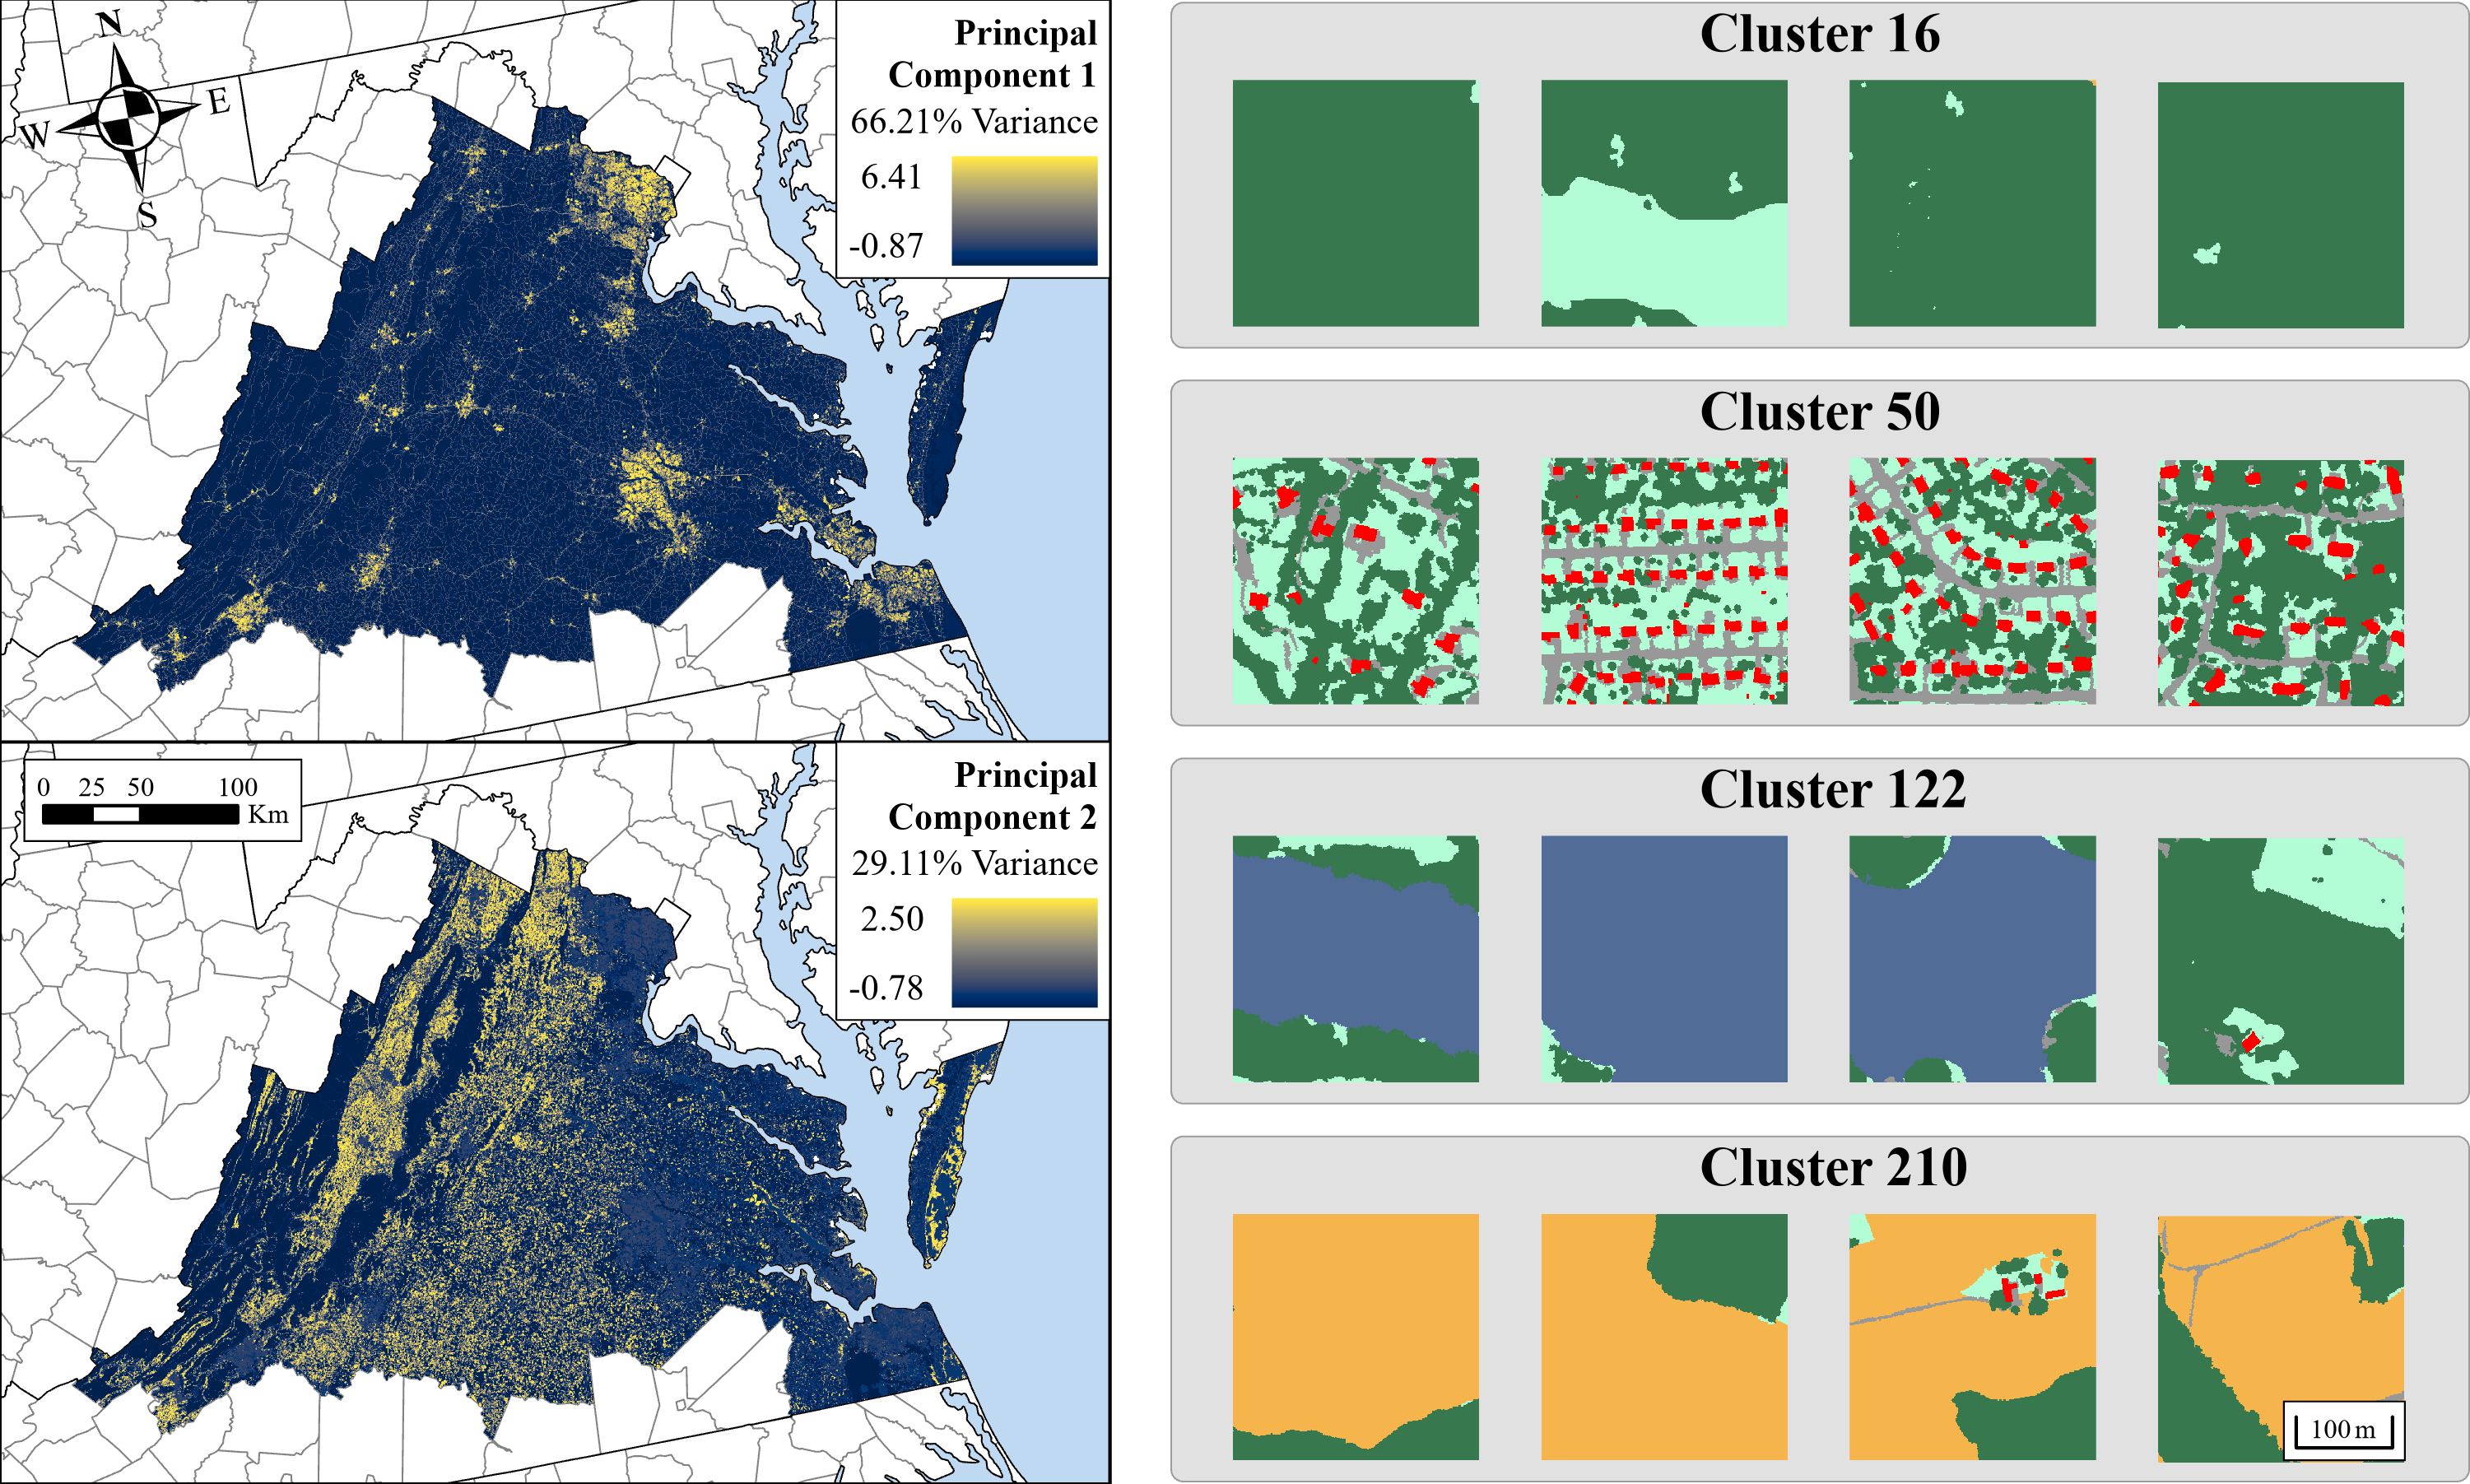
\includegraphics[width=\textwidth]{images/VA_PCs_Layout.png}
    \caption{
        Geographical distribution of principal components of land cover histograms from candidate sample tiles in the Chesapeake Bay watershed in Virginia.
    }\label{fig:va_pcs}
\end{figure}

The mIoU results for models trained using the different sampling strategies and dataset sizes according to the procedure outlined in Section~\ref{sec:methodology:semantic_stratification} are shown in Figure~\ref{fig:stratification_results}.
A two-way ANOVA test indicates that both the sampling strategy \(p < 0.001\) and training dataset size \(p < 0.001\) have a statistically significant effect on model performance, while the interaction between the two factors is not statistically significant \(p = 0.082\).
However, the Tukey HSD post-hoc test reveals that the semantic stratification strategy does not yield statistically significant improvements in mIoU at \(N_\text{train} = 250\).
Still, significant improvements in mIoU over both random sampling and spatially stratified sampling are observed at \(N_\text{train} = 500\) and \(N_\text{train} = 750\).
The largest improvements in mIoU are observed at \(N_\text{train} = 750\), where our proposed stratification method yields an average mIoU increase of \num{3.11}\% over random sampling and \num{2.50}\% over spatially stratified sampling.

\begin{figure}[H]
    \centering
    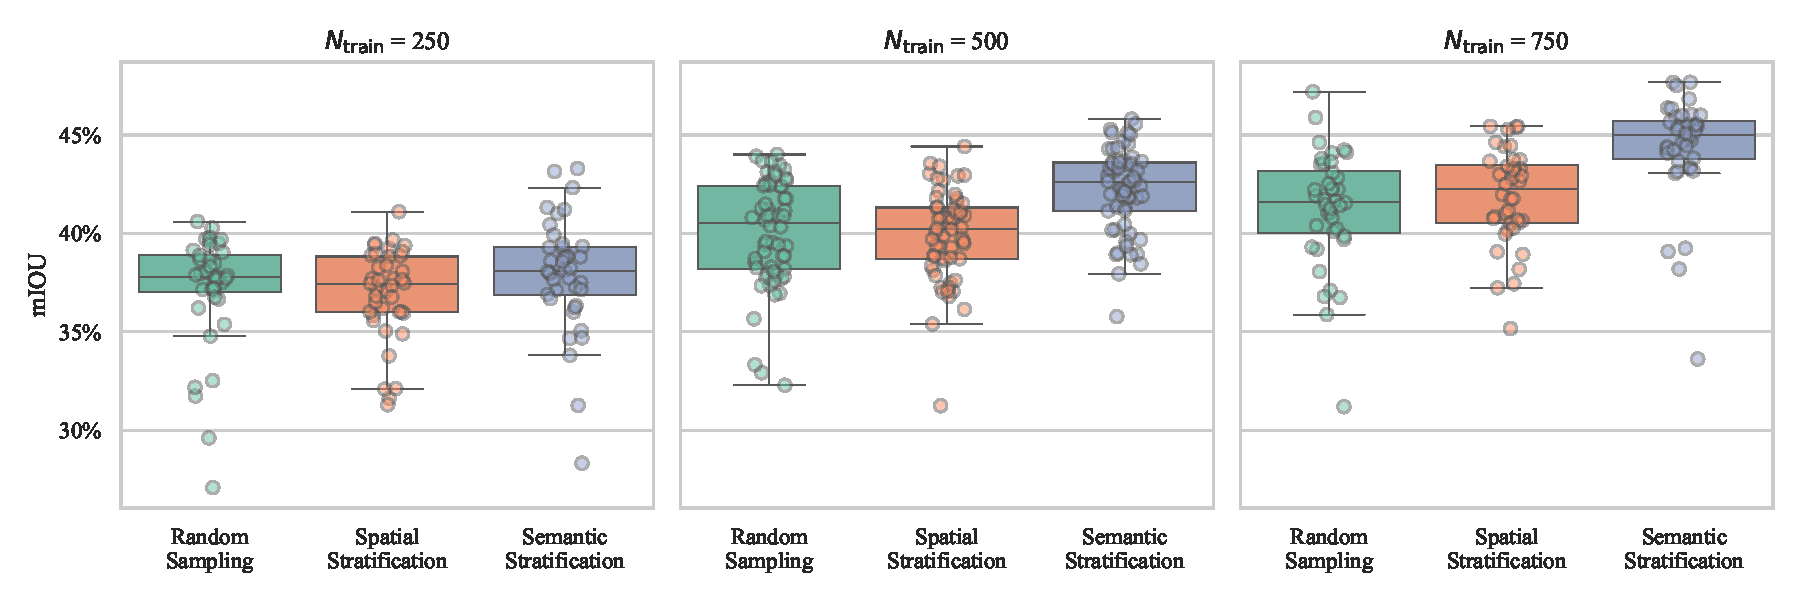
\includegraphics[width=\textwidth]{images/cpb_sampling_methods_boxplot.pdf}
    \caption{Comparison of approaches for selecting candidate patches for inclusion in the labeled training dataset across 250, 500, and 750 total labeled patches when training a DeepLabv3+ model for land cover classification.}\label{fig:stratification_results}
\end{figure}

\subsection{Evaluation of self-supervised learning approach}\label{sec:results:self_supervised_learning}

As shown in Figure~\ref{fig:probing_metrics}, using fixed embeddings from a ResNet-101 model pre-trained using BYOL as input to a linear classifer yeilds substantial improvements in mIoU over a classifier that uses embeddings from a model pre-trained only on ImageNet.
The largest training dataset size of \(N_\text{train} = 500\) yeilds the largest improvement in mIoU, with the BYOL pre-trained model achieving an mIoU of \num{41.33}\% compared to \num{32.49}\% for the ImageNet pre-trained model, an improvement of \num{8.84}\%.
Notably, the model that begins BYOL pre-training with ImageNet weights performs marginally worse than the model that begins BYOL pre-training with random weights.


\begin{figure}[H]
    \centering
    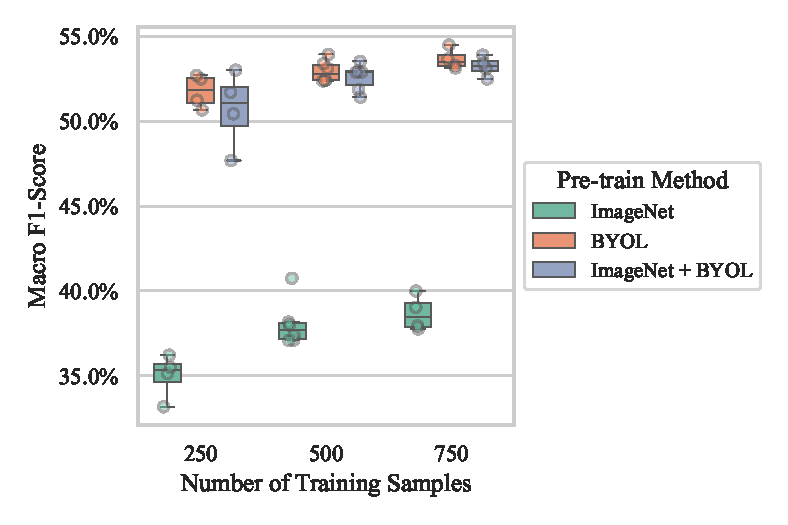
\includegraphics[width=0.6\textwidth]{images/linear_probing_results.pdf}
    \caption{Comparison of linear probing performance using features extracted by ResNet-101 backbones pre-trained with ImageNet only (green), BYOL only (orange), and ImageNet + BYOL (blue) given various amounts of labeled training data.}\label{fig:probing_metrics}
\end{figure}

This trend continues when the pre-trained ResNet-101 ba

\begin{figure}[H]
    \centering
    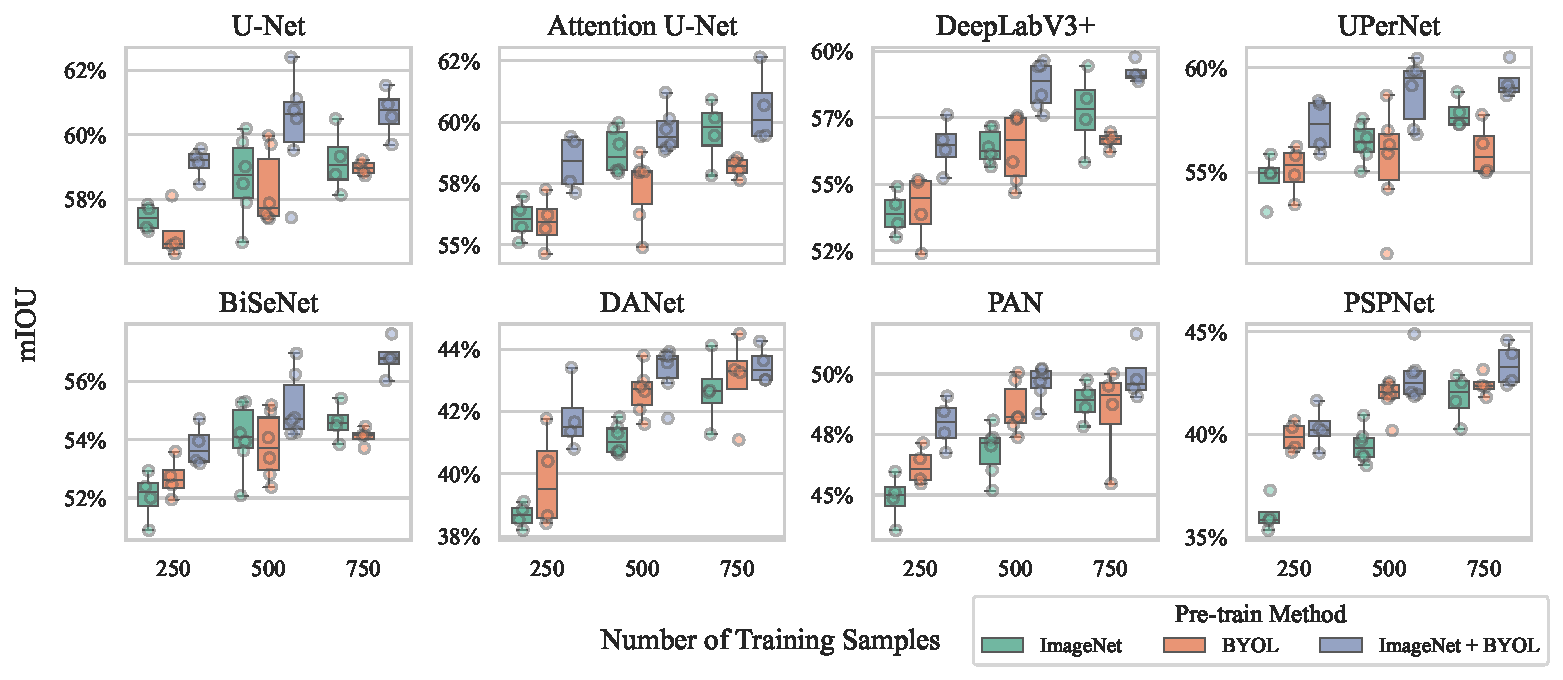
\includegraphics[width=\textwidth]{images/finetuning_results.pdf}
    \caption{Macro F1 score of semantic segmentation architectures using backbones pre-trained with ImageNet only (green), BYOL only (orange), and BYOL initialized with ImageNet weights prior to pre-training (blue) given various amounts of labeled training data.}\label{fig:finetune_metrics}
\end{figure}


\begin{table}[H]
    \centering
    \label{tab:confusion_matrix}
    \caption{Confusion matrix for the Mississippi land cover classification results.}
    \vspace{0.25cm}
    \renewcommand{\arraystretch}{1.75} % Adjust the row height
    \resizebox{\textwidth}{!}{
        \begin{tabular}{@{}|l|rrrrrrrr|r|@{}}
            \toprule
            \diagbox{\makecell{True\\Label}}{\makecell{Predicted\\Label}}           & \makecell[lb]{Open\\Water}    & \makecell[lb]{Impervious\\Structures}          & \makecell[lb]{Impervious\\Surfaces}         & \makecell[lb]{Barren\\Land}     & \makecell[lb]{Tree Canopy/\\Woody Vegetation} & \makecell[lb]{Low Vegetation/\\Herbaceous} & \makecell[lb]{Cultivated\\Crops} & \makecell[lb]{Unclassified}    & \makecell[lb]{Producer's\\Accuracy}          \\ \midrule
            {Open Water}                                     & \textbf{7154} & 344                            & 41                          & 45              & 16                           & 141                       & 0                & 1066            & 81.23\%             \\
            \makecell[l]{Impervious\\Structures}             & 13            & \textbf{20776}                 & 2041                        & 1335            & 115                          & 4891                      & 0                & 1708            & 67.28\%             \\
            \makecell[l]{Impervious\\Surfaces}               & 19            & 2590                           & \textbf{124159}             & 9058            & 1722                         & 14407                     & 13               & 3225            & 80.00\%             \\
            {Barren Land}                                    & 298           & 1964                           & 21482                       & \textbf{130287} & 2798                         & 100670                    & 24151            & 4008            & 45.61\%             \\
            \makecell[l]{Tree Canopy/\\Woody Vegetation}     & 924           & 244                            & 1403                        & 1064            & \textbf{2336744}             & 94750                     & 26166            & 101005          & 91.20\%             \\
            \makecell[l]{Low Vegetation/\\Herbaceous}        & 469           & 2596                           & 24339                       & 57498           & 58379                        & \textbf{851272}           & 136447           & 29850           & 73.33\%             \\
            {Cultivated Crops}                               & 0             & 0                              & 171                         & 3079            & 6685                         & 48908                     & \textbf{148924}  & 603             & 54.73\%             \\
            {Unclassified}                                   & 208           & 940                            & 3546                        & 384             & 14128                        & 8236                      & 106              & \textbf{147915} & 62.64\%             \\ \midrule
            {User's Accuracy}                                      & 78.75\%       & 70.54\%                        & 70.07\%                     & 64.26\%         & 96.53\%                      & 75.78\%                   & 44.34\%          & 51.11\%         & \makecell[r]{Overall Accuracy\\82.11\%}      \\ \bottomrule
        \end{tabular}
    }
\end{table}